\documentclass[11pt,a4paper,oneside]{article}
\renewcommand{\baselinestretch}{1.5} 

\usepackage{graphicx}
\usepackage{epstopdf}
\usepackage{color}
\usepackage{cite}
\usepackage{ulem}
\usepackage{subfigure}
\usepackage{bm}% bold math
\usepackage{dcolumn}% Align table columns on decimal point
\usepackage{chngcntr}

%\usepackage{pnastwoF}
\usepackage{amssymb,amsfonts,amsmath,mathrsfs}

%\addtolength{\oddsidemargin}{-0.75cm}
%\addtolength{\evensidemargin}{-2.25cm}
%\addtolength{\textwidth}{3cm}
%\addtolength{\topmargin}{-0.75cm}
%\addtolength{\textheight}{0.75cm}
\title{VESUVIO assessment}
\author{M. Krzystyniak \footnote{matthew.krzystyniak@stfc.ac.uk} and G. Romanelli \footnote{giovanni.romanelli@uniroma2.it}}

\usepackage{fullpage}

\newcommand{\ek}{ \langle E_K\rangle}
\newcommand{\tof}{ $t.o.f.$ }
\newcommand{\ie}{ {\it i.e.}, }

\begin{document}
\maketitle

\section{Calibration with no CCR}

The MANTID routine EVSCalibrationAnalysis is used in order to get a calibration of the instrument when no Al CCR is used. As a first step, the aforementioned routine can determine the values of $L_0$ and $t_0$ using:
\begin{itemize}
\item  an U foil in the sample position inside CCR (run 14025 measured by M. Adams on December 2008, 45.6 $\mu$Ah). This is used to define $L_0$ and $t_0$ from the ($n,\gamma$) resonances measured by YAP detectors in forward scattering.
\item a 2 mm Lead with U foil upstream (run 12571 measured by M. Adams on February 2008, 3129 $\mu$Ah). This is used to define $L_0$ and $t_0$ from the dips in the spectra measured by $^6$Li glass detectors in backscattering.
\item a 2 mm Lead (run 12571 measured by M. Adams on February 2008, 2799 $\mu$Ah). This is used as a background in both cases since there are no structures in the region of the resonances 120 $\mu$s $< t <$ 320 $\mu$s.
\end{itemize}
These are all old runs, but are mainly needed for quantities that should be independent on the position of the detectors. On the other hand, if the negative value for $t_0$ is due to electronics issues, there could have been major changes in the last 7 years with replacement of cables and devices. 

The other parameters to be fitted are $L_1$, $E_1$ and $\theta$. The calibration of these parameters is based\footnote{Calibration of an electron volt neutron spectrometer, Nuclear Instruments and Methods in Physics Research A (15 October 2010), doi:10.1016/j.nima.2010.09.079 by J. Mayers, M. A. Adams} on
\begin{itemize}
\item a 2 mm Lead in chimney with no CCR (runs 17687 -- 17712 measured by MK and GR on April 2015, 2340 $\mu$Ah). d-spacing is used for $\theta$ and $L_1$ and the position of the recoiling peak for $E_1$ and $L_1$.
\item a V slab as a background (run 17086 measured by A. Seel on April 2014, 1509 $\mu$Ah).
\end{itemize}

The procedure is iterate twice and convergence for the parameters is obtained. The iterative procedure is initialised by an input consisting of an old instrument parameter file.



\section{Dependence of the results on the initialising parameters}

Three Instrument Parameter (IP) files have been used in order to initialise the calibration routine: Ip0004, Ip0005 and a mechanically-measured list of parameters denoted as IpSurvey. All considered initialising IP files where calibrated in CCR. $L_0$ assumed the same value for all the initialising files: $L_0=11.005$ m, and after the calibration it is again the same in the three outputs: $L_0=11.0047$ m, that is the value is unchanged. Simultaneously, the value for $t_0$ is obtained for all the detectors. In Figure \ref{t0}, the values for the three outputs are reported. While the value for $t_0$ is defined in the calibration algorithm as shared by all front-scattering detectors ($t_0=-0.196$), it is individually defined for the backscattering detectors. The mean value on the distribution of backscattering detectors seems also different (and lower) than that on front-scattering detectors. The standard deviations for each detector are evaluated on the ensemble of the values form the three calibrations and reported in the same Figure  \ref{t0} showing not-appreciable differences for all detectors but detector 55. The values of $t_0$ for front-scattering detectors reported in IP files IP2572 (2008), IP004 (2013) and IP005 (2014) are respectively -0.52 $\mu$s, -0.40 $\mu$s and -0.32 $\mu$s. The value just measured confirms a trend of decrease year-after-year.  

The values for $L_1$ resulting from the calibration procedure are reported in Figure \ref{L1} and are presented as the deviation with respect to the mechanically-measured value from  the IpSurvey. An almost constant offset of 2 cm is found for all detectors in both front- and backscattering: he mean position for the photon or neutron detection is different from the front face of the YAP detectors or from the centre of the $^6$Li glasses. With the exception of few detectors, the values for the three calibrations are so similar that the standard deviations are not appreciable. The differences between the initialising and resulting values in the case of IP0005 are also reported. The difference is appreciable and of about 1 cm.

In Figure \ref{theta}, the values for $\theta$ are presented as the deviation with respect to the mechanically-measured value from  the IpSurvey. With the exception of few detectors, the values for the three calibrations are so similar that the standard deviations are not appreciable. While the values of $\theta$ are generally underestimated by 2 degrees with respect to the survey values in backscattering, in the case of front-scattering they are overestimated by about 1 degree. The differences between the initialising and resulting values in the case of IP0005 are also reported. The difference is appreciable and of about 1 degree for backscattering detectors.

\begin{figure}
\centering
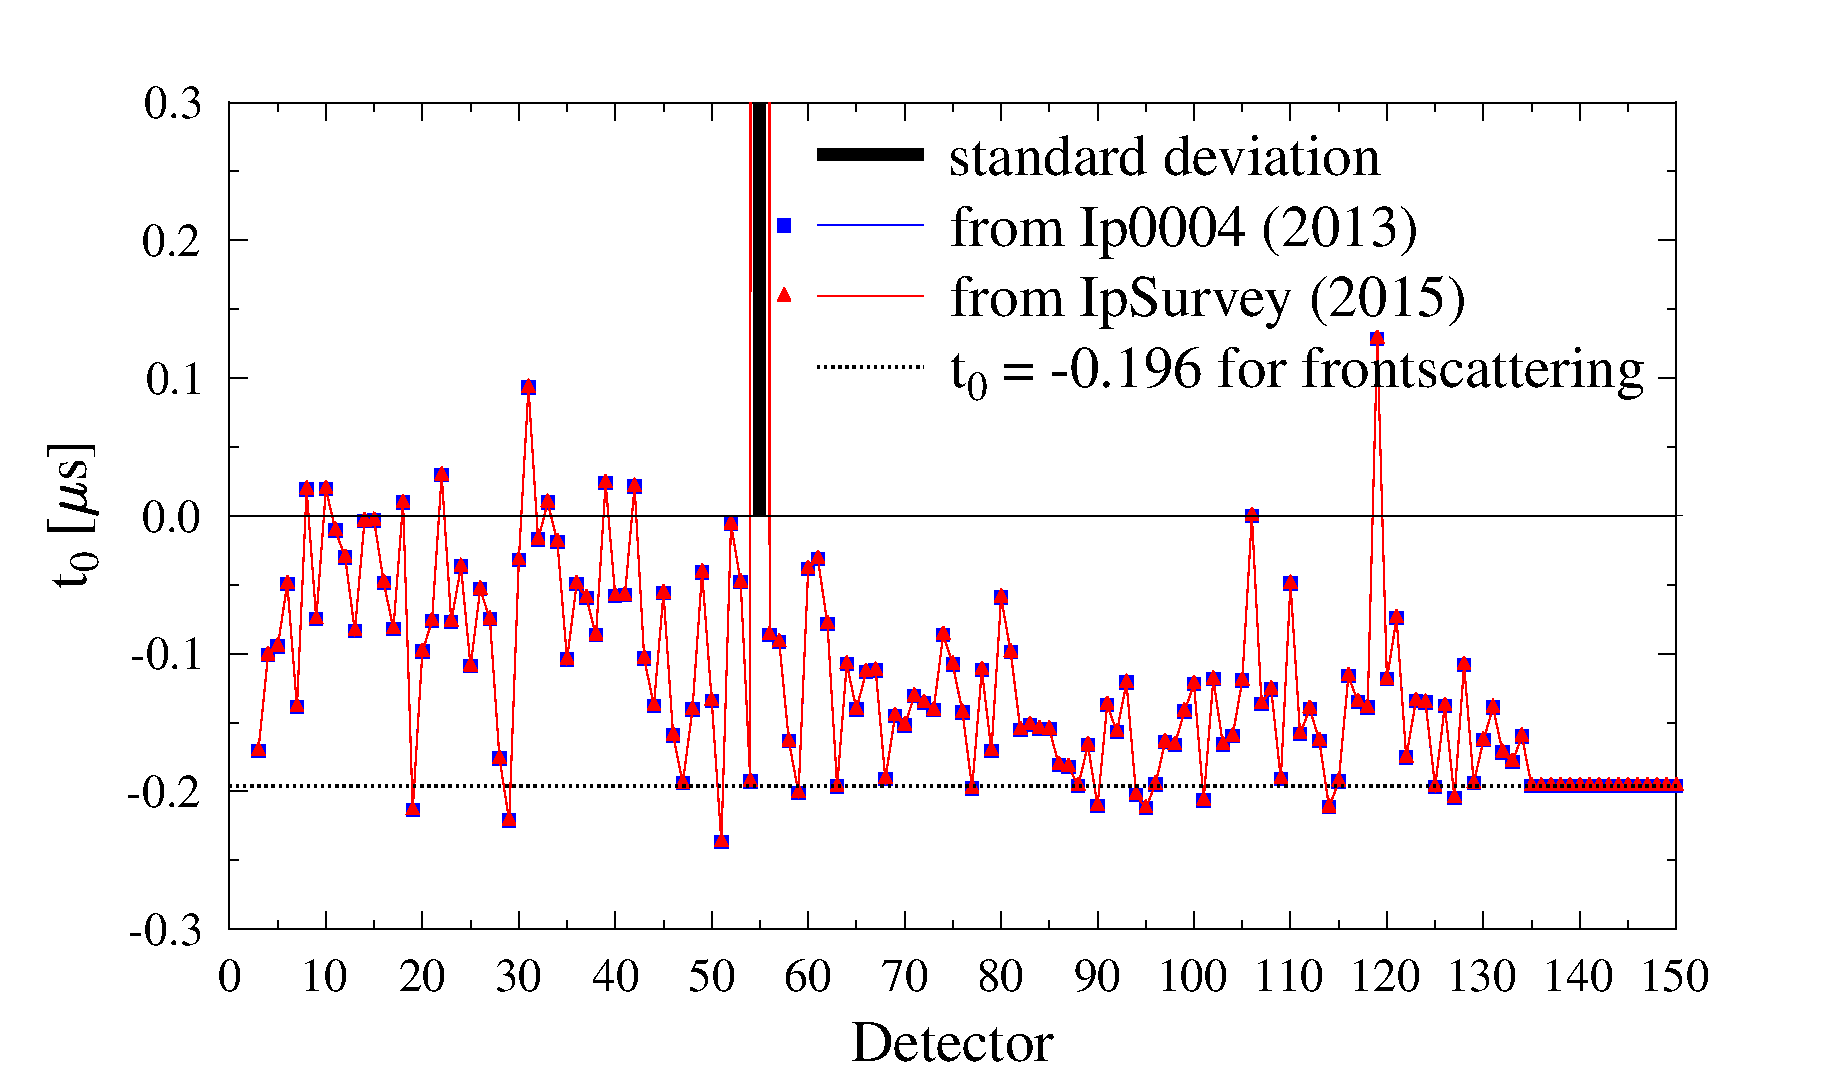
\includegraphics[width=\textwidth]{img/t0}
\caption{Values of $t_0$ after the calibration from different initialising IP files. The values from  IP0005 are the same as those from IP0004 and have not been reported. The standard deviations for each detector are evaluated on the ensemble of the values form the three calibrations. Detector 55 has an anomalous values of $t_0(Ip0004)= 36.5051$ $\mu$s and	$t_0(IpSurvey)=33.6723$ $\mu$s. Detector 106 has all the values identically null. Differences between the values from different IP files are of the order of 10$^{-5}$ $\mu$s.}
\label{t0}
\end{figure}



\begin{figure}
\centering
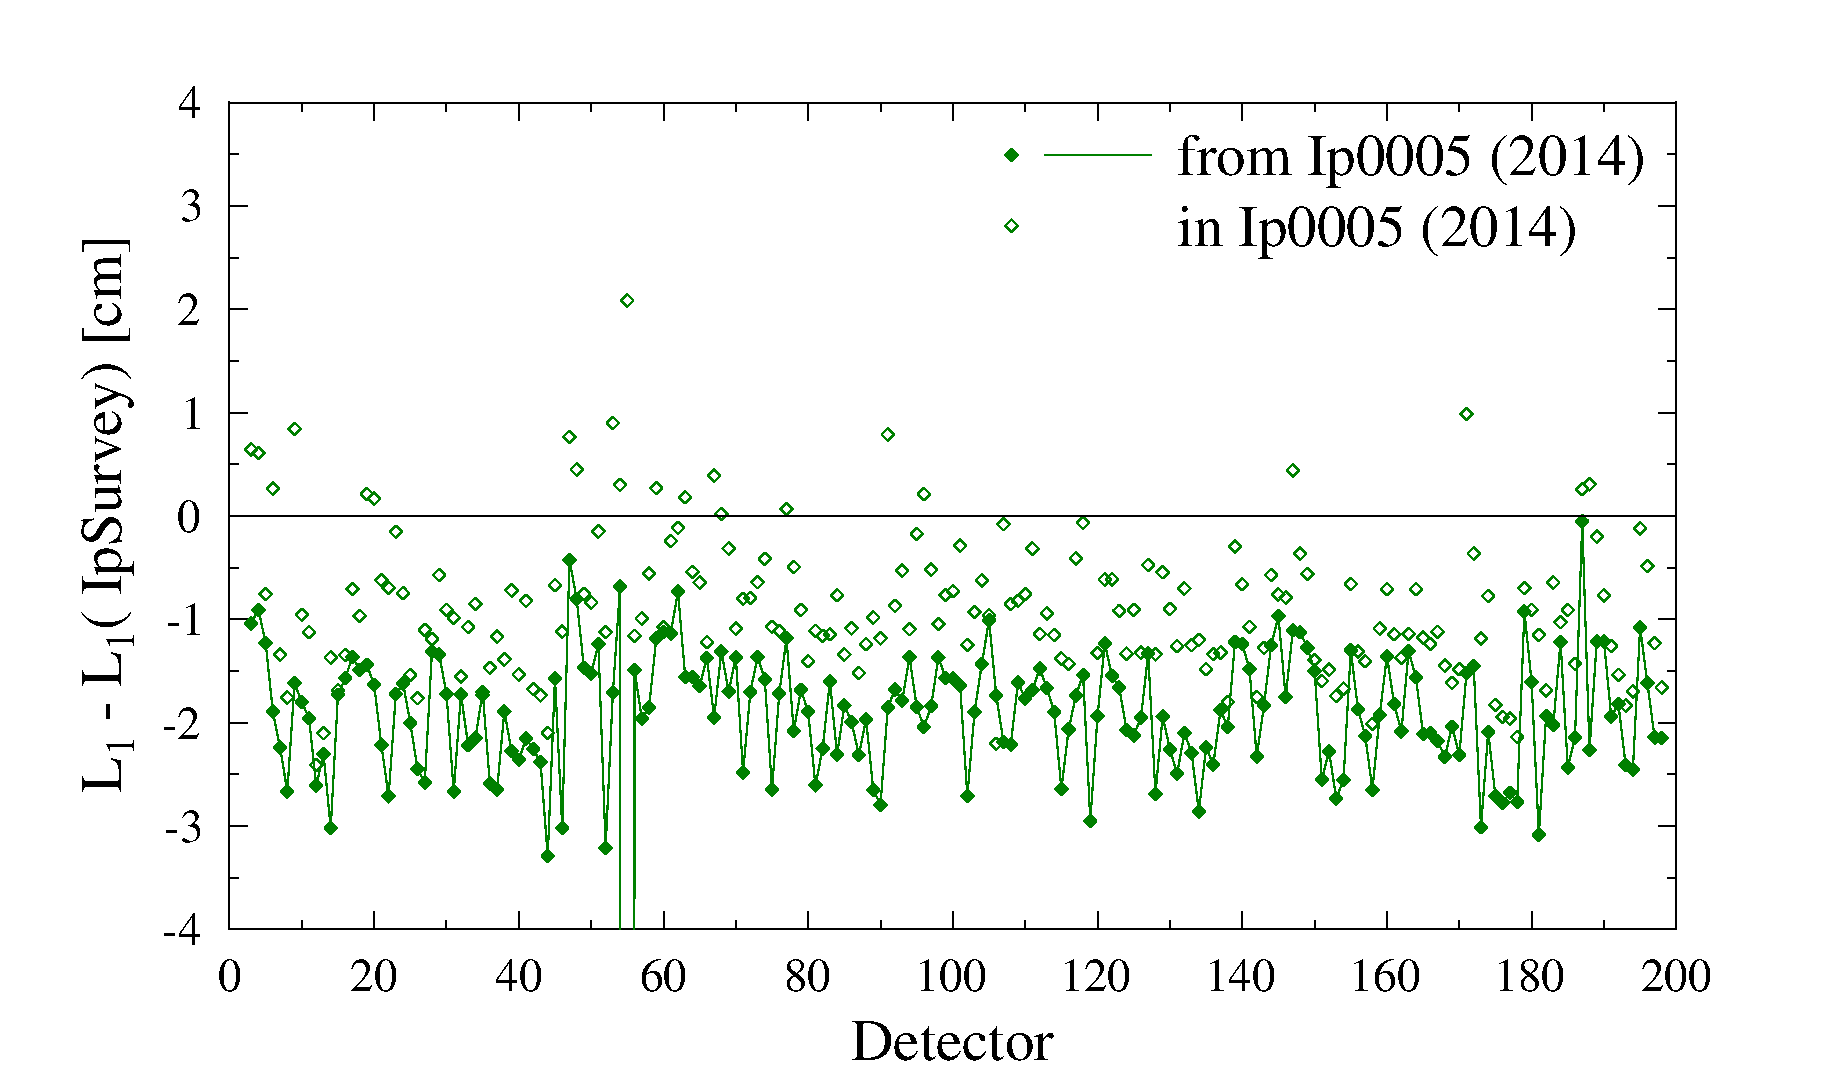
\includegraphics[width=\textwidth]{img/L1_bis}

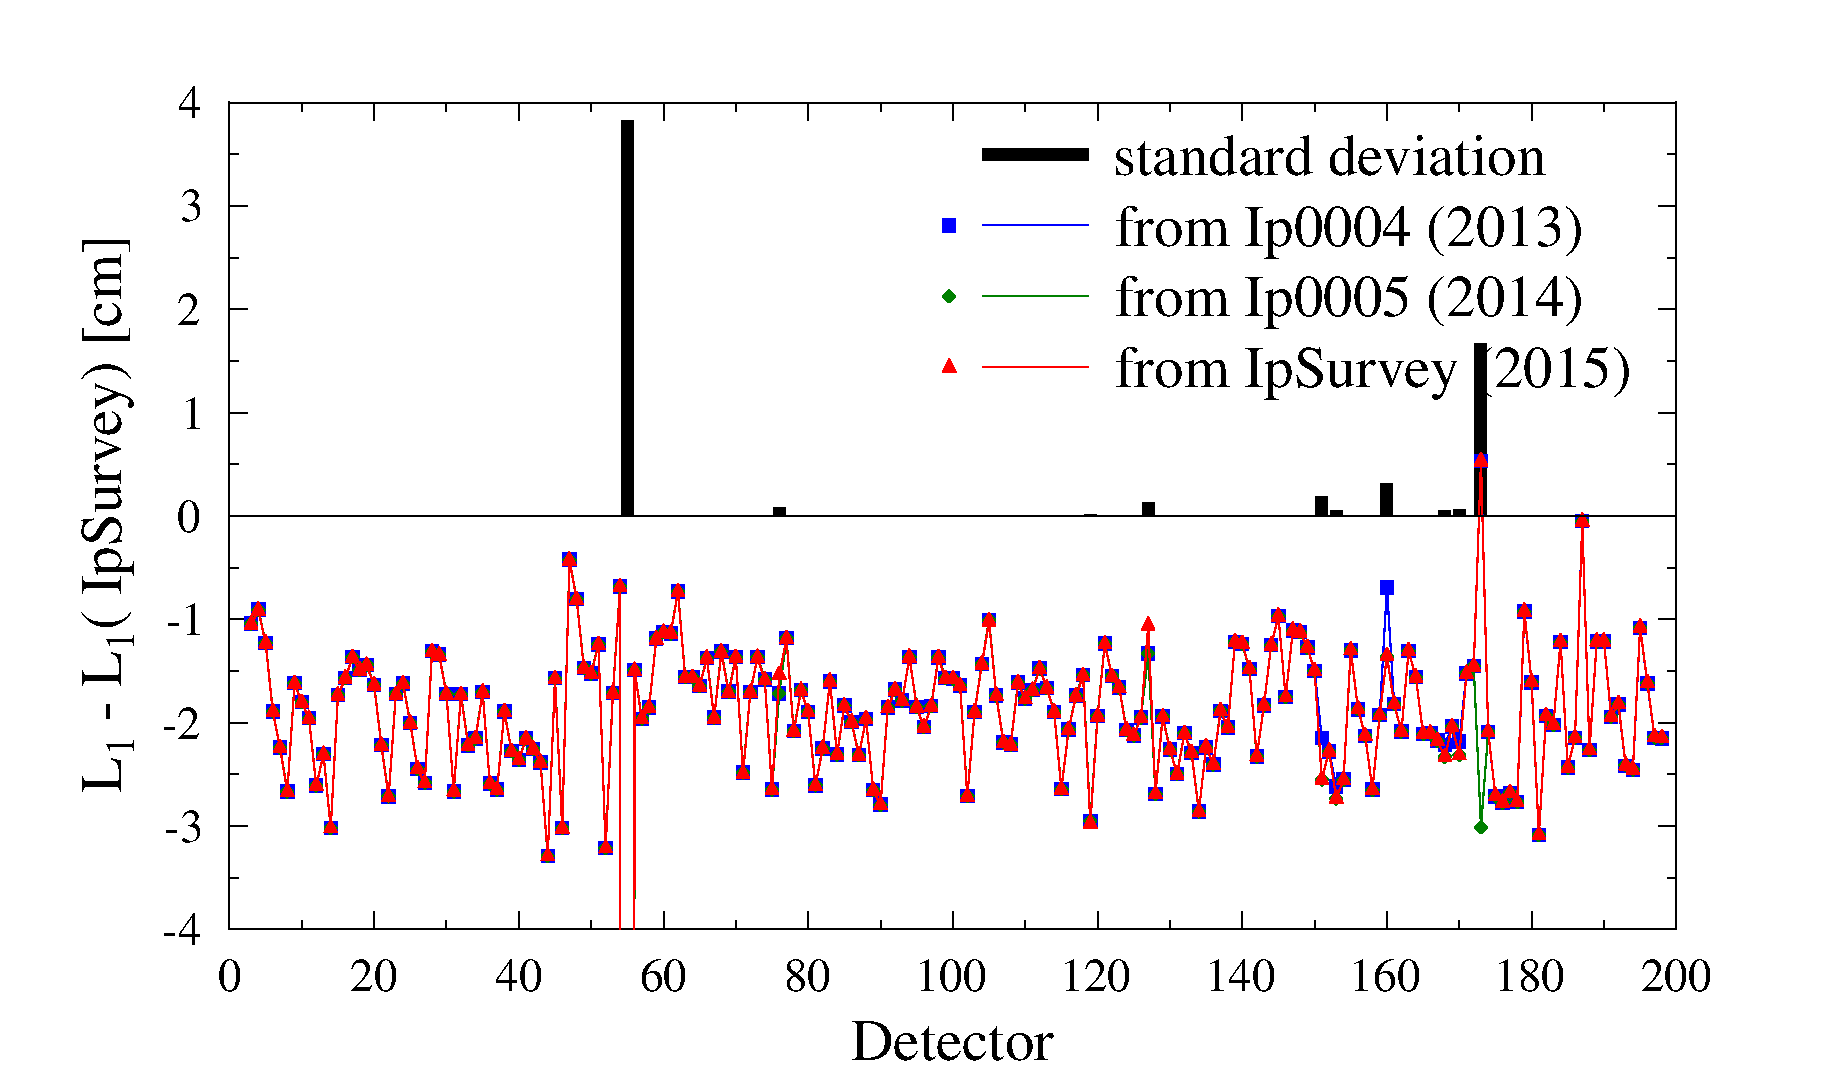
\includegraphics[width=\textwidth]{img/L1}
\caption{Values of $L_1$ after the calibration from different initialising IP files. The mechanically-measured values in IpSurvey are used as the offset. The standard deviations for each detector are evaluated on the ensemble of the values form the three calibrations. The two largest discrepancies are for detectors 55 and 173.}
\label{L1}
\end{figure}


\begin{figure}
\centering
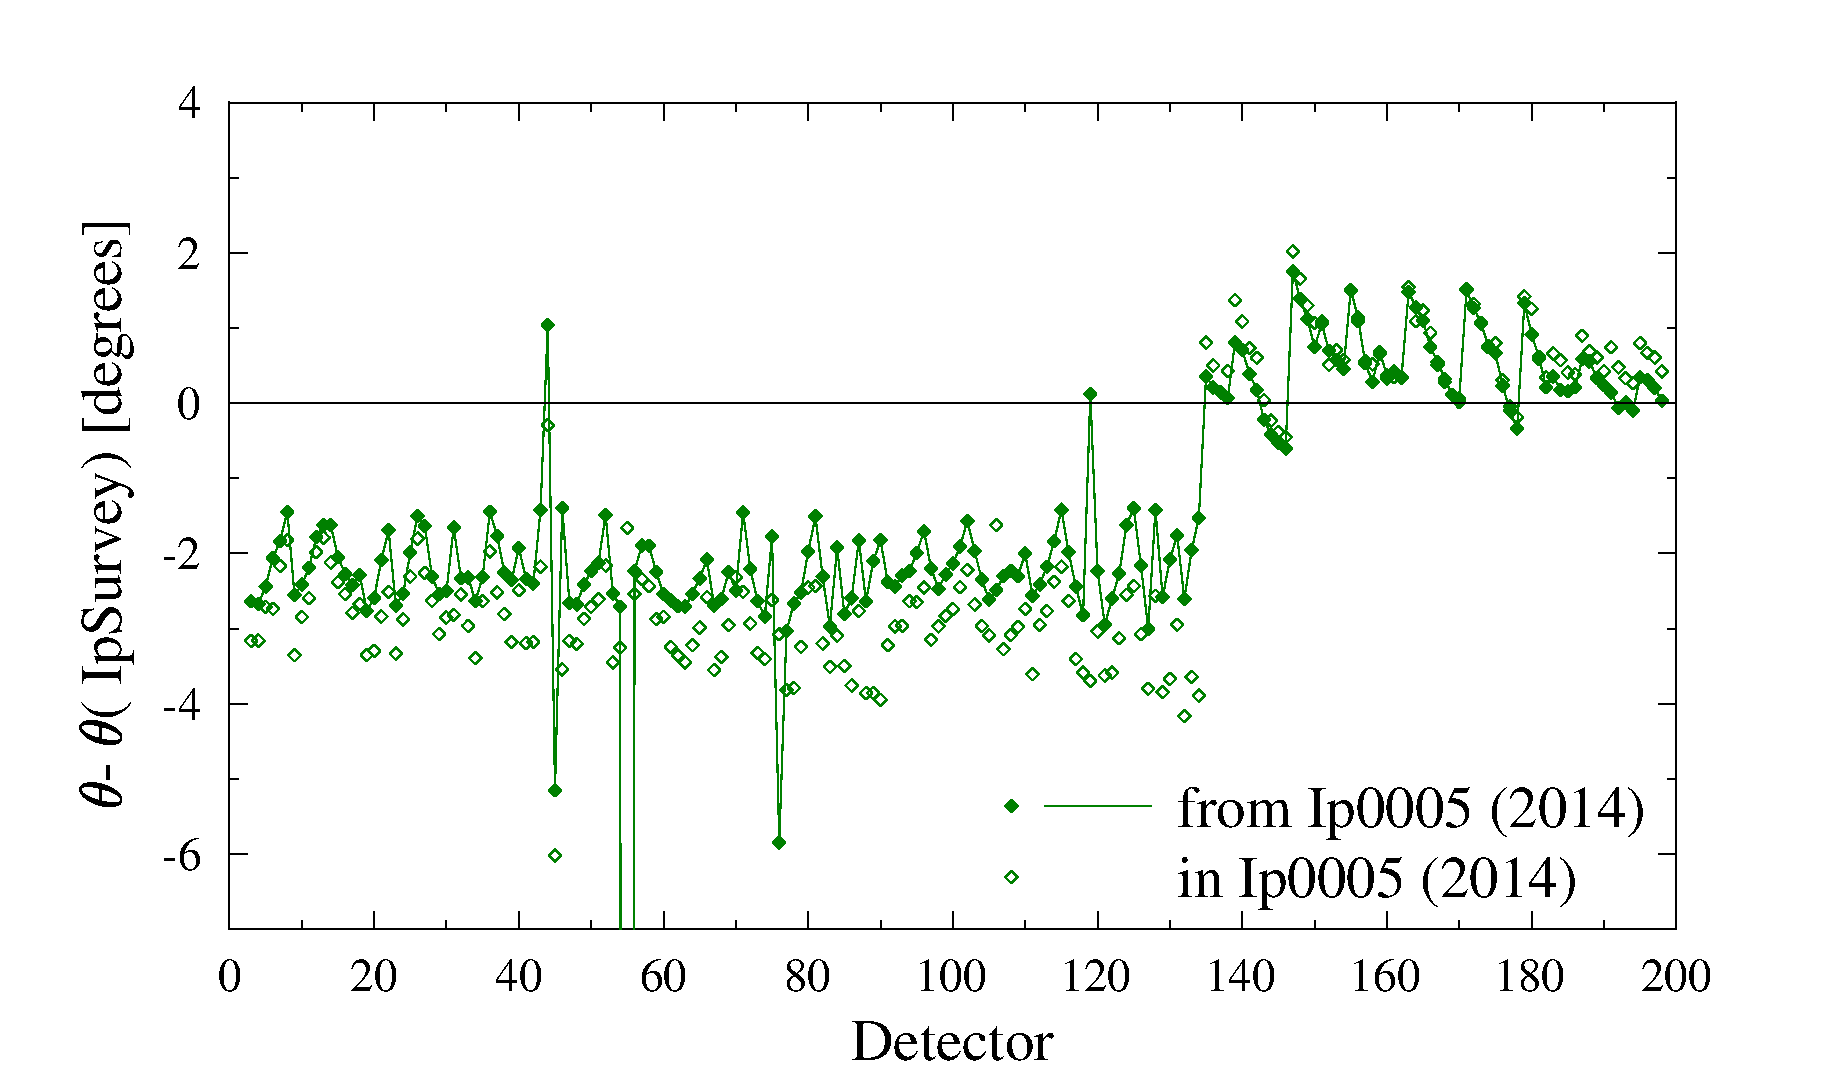
\includegraphics[width=\textwidth]{img/theta_bis}

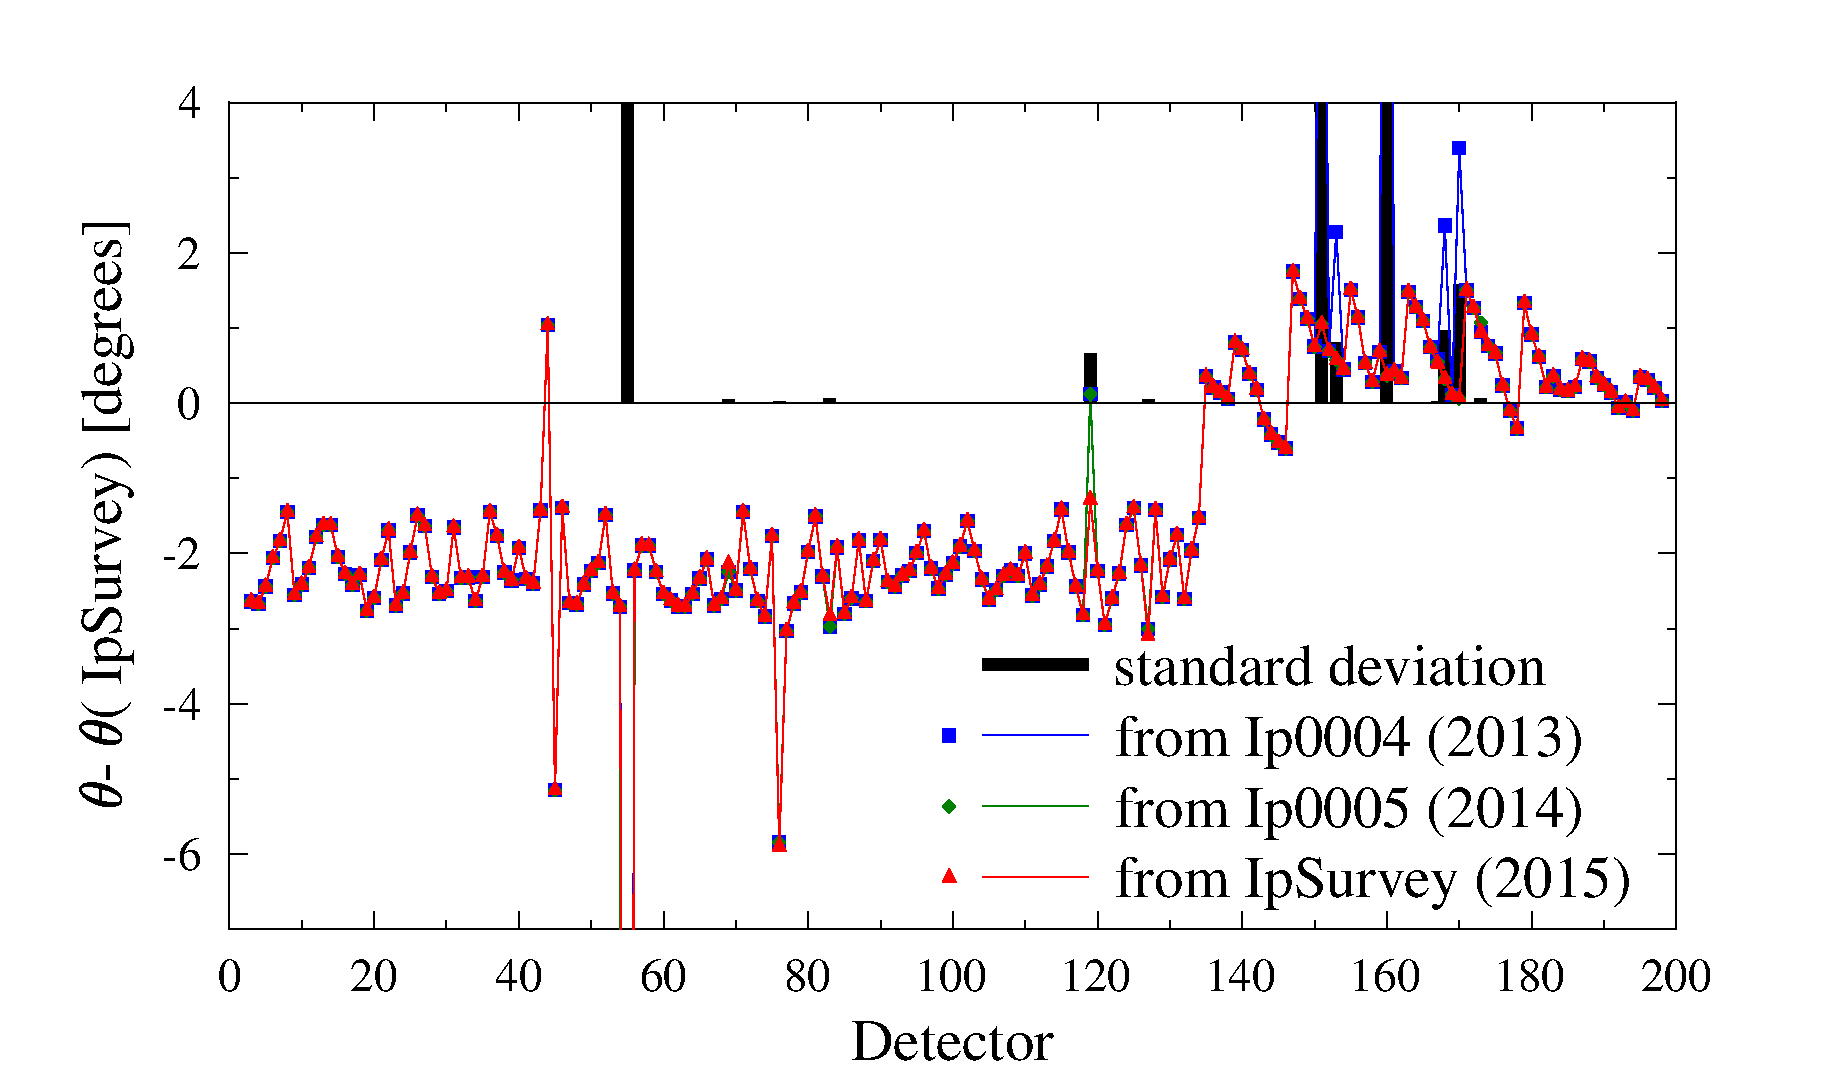
\includegraphics[width=\textwidth]{img/theta}
\caption{Values of $\theta$ after the calibration from different initialising IP files. The mechanically-measured values in IpSurvey are used as the offset. The standard deviations for each detector are evaluated on the ensemble of the values form the three calibrations. The largest discrepancies are found for detectors 55, 119, 151, 153, 160, 168 and 170.}
\label{theta}
\end{figure}



\section{Comments}

\begin{itemize}
\item U-foil on sample position with no CCR, 2 mm Pb with U-foil upstream and with no CCR and V slab with no CCR are needed for upgrade
\item Why are we using vanadium as a background instead of lead 2mm?
\item we should add an option to take ENERGY\_ESTIMATE = constant for the calibration.
\item Do we expect different values of $t_0$ between front- and backscattering and between old and new calibrations?
\end{itemize}

\begin{figure}
\centering
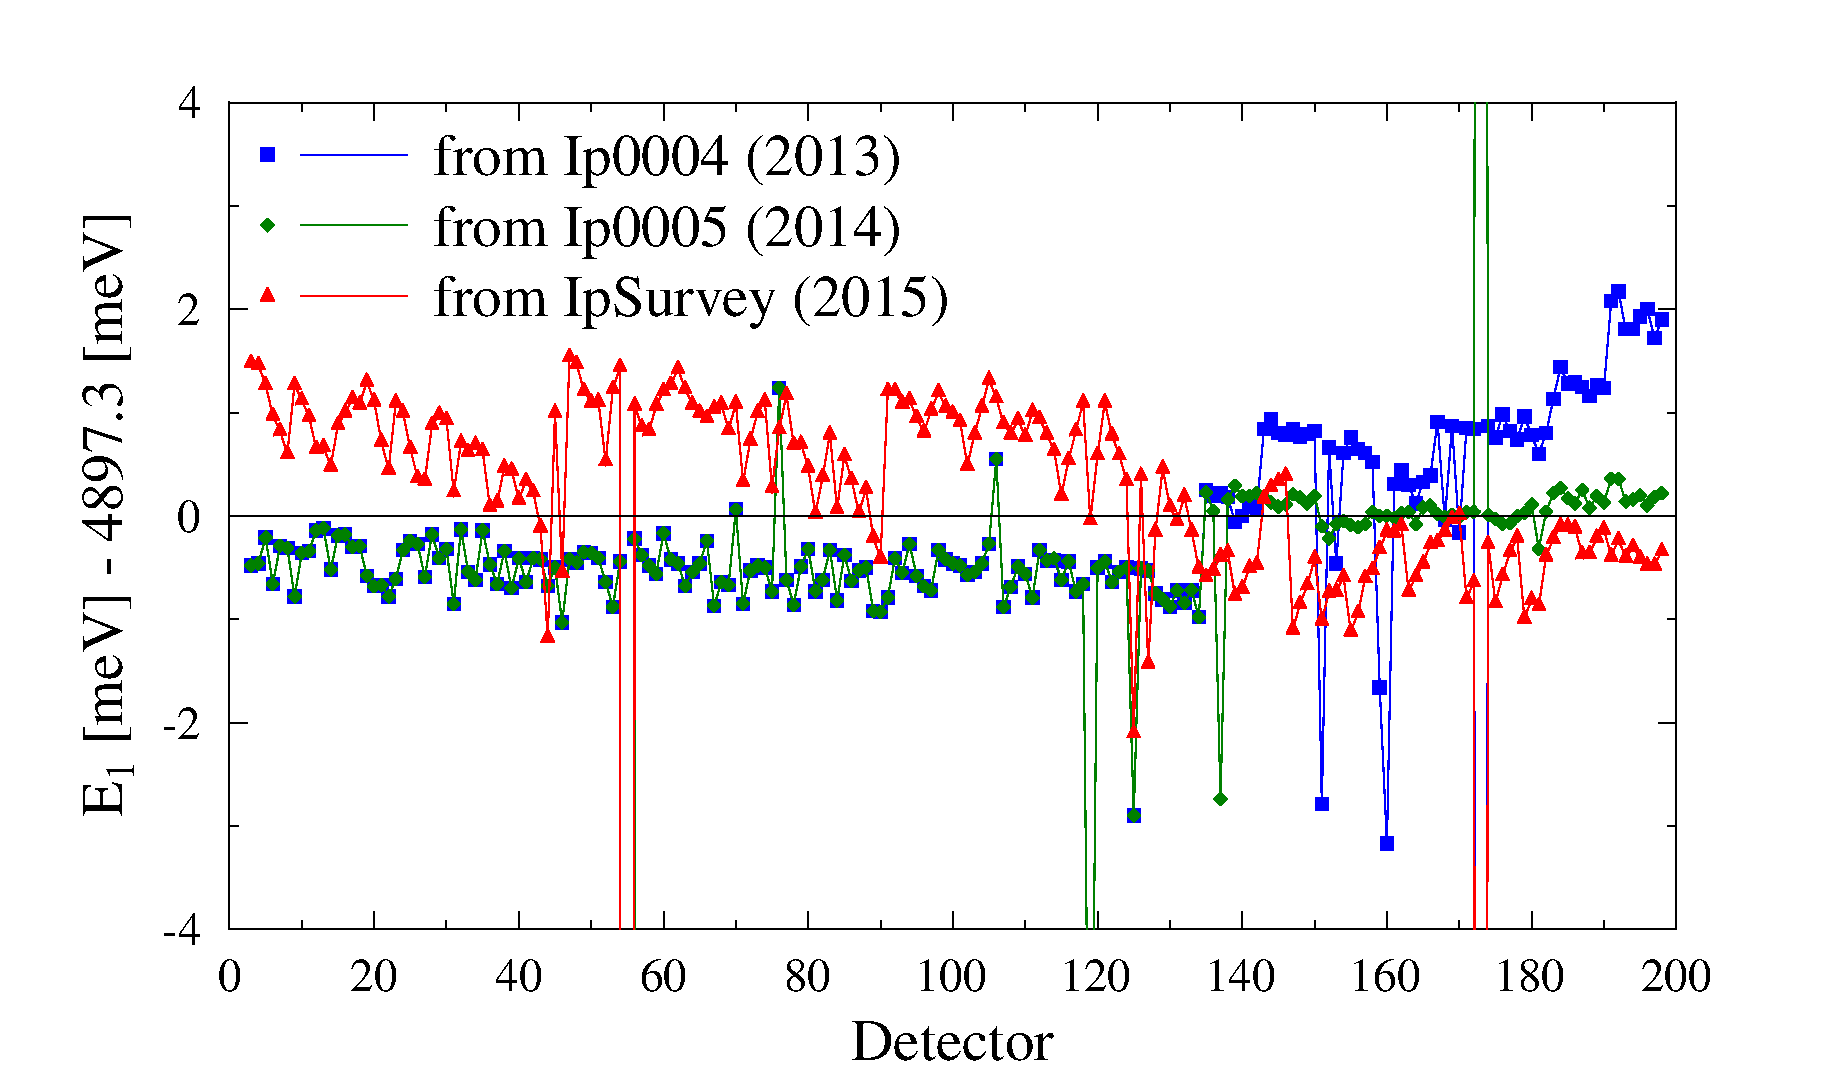
\includegraphics[width=\textwidth]{img/E1}
\caption{Values of $E_1$ after the calibration from different initialising IP files. Values are presented as offset with respect to the published value of $E_1=4897.3$ meV. The largest discrepancies are found for detectors 55, 119, 137 151, 160 and 173.}
\label{t0}
\end{figure}

\end{document}








%
%\begin{document}\bibliography{bibliotesi}











